\documentclass[11pt,a4paper]{article}

\usepackage[utf8]{inputenc}
\usepackage[T1]{fontenc}
\usepackage[english]{babel}
\usepackage{amsmath,amssymb,mathtools}
\usepackage{graphicx}
\usepackage{booktabs,longtable,array}
\usepackage{geometry}
\usepackage{float}
\usepackage{enumitem}
\usepackage{xcolor}
\usepackage{listings}
\usepackage{hyperref}
\usepackage{microtype}
\usepackage{fancyhdr}
\usepackage{caption}

\geometry{margin=2.1cm}
\setlength{\parindent}{0pt}
\setlength{\parskip}{5pt}
\setlist[enumerate]{itemsep=5pt,topsep=4pt}
\hypersetup{colorlinks=true,linkcolor=blue!50!black,urlcolor=blue!50!black}
\pagestyle{fancy}
\setlength{\headheight}{14pt}
\fancyhf{}
\lhead{Introductory Econometrics}
\rhead{Tutorial 1}
\cfoot{\thepage}
\captionsetup{font=small}

\definecolor{codegray}{gray}{0.96}
\lstset{
  basicstyle=\ttfamily\footnotesize,
  backgroundcolor=\color{codegray},
  frame=single,
  breaklines=true,
  columns=fullflexible,
  keepspaces=true,
  showstringspaces=false
}

\newcommand{\E}{\mathbb{E}}
\newcommand{\Var}{\operatorname{Var}}
\newcommand{\Cov}{\operatorname{Cov}}
\newcommand{\SSR}{\mathrm{SSR}}
\newcommand{\Sxx}{S_{xx}}

\title{\textbf{Tutorial 1 -- OLS Mechanics and Interpretation}\\
\large Complete Theory Solutions and Python Lab Outputs}
\author{Introductory Econometrics -- Telecom Paris}
\date{September 2026}

\begin{document}
\maketitle
\tableofcontents
\newpage

\section{Theory Exercises}

\subsection{Exercise 1 -- Deriving OLS}
Consider the simple regression model
\[
 y_i=\beta_0+\beta_1x_i+u_i, \qquad i=1,\ldots,n.
\]

\subsubsection*{(a) Sum of squared residuals and first-order conditions}
For arbitrary candidate coefficients $(b_0,b_1)$, the residual for observation $i$ is
\[
 e_i(b_0,b_1)=y_i-b_0-b_1x_i.
\]
OLS chooses $(\hat\beta_0,\hat\beta_1)$ to minimize
\[
 S(b_0,b_1)=\sum_{i=1}^n (y_i-b_0-b_1x_i)^2.
\]
The first-order condition with respect to $b_0$ is
\[
 \frac{\partial S}{\partial b_0}
 =-2\sum_{i=1}^n(y_i-b_0-b_1x_i)=0,
\]
so at the OLS solution,
\[
 \boxed{\sum_{i=1}^n \hat u_i=0}.
\]
The first-order condition with respect to $b_1$ is
\[
 \frac{\partial S}{\partial b_1}
 =-2\sum_{i=1}^n x_i(y_i-b_0-b_1x_i)=0,
\]
so
\[
 \boxed{\sum_{i=1}^n x_i\hat u_i=0}.
\]

\subsubsection*{(b) OLS intercept and slope}
From the first condition,
\[
 0=\sum_i(y_i-\hat\beta_0-\hat\beta_1x_i)
 =n\bar y-n\hat\beta_0-n\hat\beta_1\bar x,
\]
therefore
\[
 \boxed{\hat\beta_0=\bar y-\hat\beta_1\bar x}.
\]
Substituting this into the second first-order condition gives
\[
 \sum_i (x_i-\bar x)(y_i-\bar y)
 =\hat\beta_1\sum_i(x_i-\bar x)^2.
\]
Hence
\[
 \boxed{
 \hat\beta_1=
 \frac{\sum_i(x_i-\bar x)(y_i-\bar y)}
 {\sum_i(x_i-\bar x)^2}
 }.
\]
The slope exists and is uniquely identified when
\[
 \boxed{\Sxx=\sum_i(x_i-\bar x)^2>0},
\]
meaning that the sample contains variation in $x$; the $x_i$ cannot all be equal.

\subsubsection*{(c) Sample analogues of the population moment conditions}
The population conditions are
\[
 \E(u)=0, \qquad \E(xu)=0.
\]
Their sample analogues replace expectations by sample averages and the unobserved population error by the OLS residual:
\[
 \frac{1}{n}\sum_i\hat u_i=0,
 \qquad
 \frac{1}{n}\sum_i x_i\hat u_i=0.
\]
Multiplying by $n$ gives exactly the two OLS first-order conditions derived above.

\subsubsection*{(d) Mechanical OLS identities}
The first-order conditions directly imply
\[
 \boxed{\sum_i\hat u_i=0},
 \qquad
 \boxed{\sum_i x_i\hat u_i=0}.
\]
Moreover,
\[
 0=\bar{\hat u}=\bar y-\hat\beta_0-\hat\beta_1\bar x,
\]
so
\[
 \boxed{\bar y=\hat\beta_0+\hat\beta_1\bar x}.
\]
Thus the fitted OLS line passes through $(\bar x,\bar y)$. These facts are \emph{not} evidence that the population assumptions are correct: they hold mechanically because OLS chooses the coefficients to satisfy the sample first-order conditions.

\subsection{Exercise 2 -- Unbiasedness and Failure of Exogeneity}
Let
\[
 \Sxx=\sum_i(x_i-\bar x)^2.
\]

\subsubsection*{(a) Decomposition of the OLS slope}
Start from the centered-sums formula:
\[
 \hat\beta_1
 =\frac{\sum_i(x_i-\bar x)(y_i-\bar y)}{\Sxx}.
\]
Since $\sum_i(x_i-\bar x)=0$,
\[
 \sum_i(x_i-\bar x)(y_i-\bar y)
 =\sum_i(x_i-\bar x)y_i.
\]
Substitute $y_i=\beta_0+\beta_1x_i+u_i$:
\begin{align*}
 \hat\beta_1
 &=\frac{\sum_i(x_i-\bar x)(\beta_0+\beta_1x_i+u_i)}{\Sxx}\\
 &=\frac{\beta_0\sum_i(x_i-\bar x)
 +\beta_1\sum_i(x_i-\bar x)x_i
 +\sum_i(x_i-\bar x)u_i}{\Sxx}.
\end{align*}
The first term is zero, and
\[
 \sum_i(x_i-\bar x)x_i
 =\sum_i(x_i-\bar x)^2=\Sxx.
\]
Therefore
\[
 \boxed{
 \hat\beta_1
 =\beta_1+\frac{\sum_i(x_i-\bar x)u_i}{\Sxx}
 }.
\]

\subsubsection*{(b) Conditional unbiasedness of the slope}
Condition on the complete regressor sample $X=(x_1,\ldots,x_n)$. Then the $x_i$, $\bar x$, and $\Sxx$ are fixed. Hence
\begin{align*}
 \E(\hat\beta_1\mid X)
 &=\beta_1+
 \frac{\sum_i(x_i-\bar x)\E(u_i\mid X)}{\Sxx}.
\end{align*}
Under the zero conditional mean assumption (SLR.4),
\[
 \E(u_i\mid X)=0,
\]
so
\[
 \boxed{\E(\hat\beta_1\mid X)=\beta_1}.
\]
It is precisely the zero conditional mean assumption that makes the numerator have conditional mean zero.

\subsubsection*{(c) Conditional unbiasedness of the intercept}
Using $\hat\beta_0=\bar y-\hat\beta_1\bar x$ and
\[
 \bar y=\beta_0+\beta_1\bar x+\bar u,
\]
we obtain
\[
 \hat\beta_0-\beta_0
 =\bar u-(\hat\beta_1-\beta_1)\bar x.
\]
Conditional on $X$,
\[
 \E(\bar u\mid X)=0,
 \qquad
 \E(\hat\beta_1-\beta_1\mid X)=0.
\]
Therefore
\[
 \boxed{\E(\hat\beta_0\mid X)=\beta_0}.
\]

\subsubsection*{(d) Failure of exogeneity}
Suppose instead that
\[
 \E(u_i\mid X)=\rho x_i.
\]
Then
\begin{align*}
 \E(\hat\beta_1\mid X)
 &=\beta_1+
 \frac{\sum_i(x_i-\bar x)\rho x_i}{\Sxx}\\
 &=\beta_1+\rho
 \frac{\sum_i(x_i-\bar x)x_i}{\Sxx}\\
 &=\boxed{\beta_1+\rho}.
\end{align*}
If additionally $\E(x_i)=0$, then $\E(u_i)=\rho\E(x_i)=0$ and
\begin{align*}
 \Cov(x_i,u_i)
 &=\E(x_iu_i)-\E(x_i)\E(u_i)\\
 &=\E\!\left[x_i\E(u_i\mid x_i)\right]\\
 &=\rho\E(x_i^2)
 =\boxed{\rho\Var(x_i)}.
\end{align*}

\subsubsection*{(e) Omitted ability in a wage regression}
Suppose the true wage equation contains ability:
\[
 wage_i=\beta_0+\beta_1 educ_i+\gamma ability_i+\varepsilon_i,
 \qquad \gamma>0.
\]
If ability is omitted, it becomes part of the regression error. If ability is also positively related to education, then high-education observations tend to have positive omitted components in the error. Consequently the covariance term in the slope decomposition tends to be positive, so the estimated education slope is biased upward relative to the partial effect $\beta_1$.

\subsection{Exercise 3 -- Unbiasedness and Precision}
Let $Y_1,\ldots,Y_{10}$ be a random sample with $\E(Y_i)=\mu=2$ and $\Var(Y_i)=\sigma^2=1$. Consider
\[
 \tilde\mu_1=Y_1,
 \qquad
 \tilde\mu_2=\bar Y.
\]

\subsubsection*{(a) Unbiasedness}
For the first estimator,
\[
 \E(\tilde\mu_1)=\E(Y_1)=\mu=2.
\]
For the sample mean,
\[
 \E(\tilde\mu_2)
 =\E\!\left(\frac{1}{10}\sum_{i=1}^{10}Y_i\right)
 =\frac{1}{10}\sum_{i=1}^{10}\E(Y_i)
 =\mu=2.
\]
Thus
\[
 \boxed{\tilde\mu_1\text{ and }\tilde\mu_2\text{ are both unbiased}.}
\]

\subsubsection*{(b) Variances and precision}
\[
 \Var(\tilde\mu_1)=\Var(Y_1)=1.
\]
By independence,
\[
 \Var(\tilde\mu_2)
 =\Var(\bar Y)
 =\frac{1}{10^2}\sum_{i=1}^{10}\Var(Y_i)
 =\frac{10}{100}
 =0.1.
\]
Therefore
\[
 \boxed{\Var(\tilde\mu_1)=1,\qquad \Var(\tilde\mu_2)=0.1.}
\]
The sample mean has ten times smaller variance, so it is ten times more precise in the variance sense. Its standard deviation is $\sqrt{0.1}\approx0.316$, compared with $1$ for $Y_1$.

\subsubsection*{(c) Simulation of 20 samples from $N(2,1)$}
Using the supplied random seed, the 20 simulated values are:

\begin{center}
\begin{tabular}{r@{\qquad}rr}
\toprule
Sample & $Y_1$ & $\bar Y$\\
\midrule
1 & 2.3047 & 1.6644\\
2 & 2.8794 & 2.2697\\
3 & 1.8151 & 2.1163\\
4 & 4.1416 & 2.1026\\
5 & 2.7433 & 2.3030\\
6 & 2.2891 & 1.9357\\
7 & 0.3171 & 2.0091\\
8 & 0.7243 & 1.8049\\
9 & 2.4568 & 1.8812\\
10 & 2.6654 & 1.4104\\
11 & 1.6218 & 1.7987\\
12 & 2.4344 & 1.9792\\
13 & 0.9765 & 2.0635\\
14 & 1.6102 & 2.2222\\
15 & 2.4144 & 1.6802\\
16 & 1.8414 & 1.7788\\
17 & 1.0349 & 2.0671\\
18 & 1.3452 & 1.8912\\
19 & 3.3060 & 2.3427\\
20 & 3.7237 & 2.0701\\
\bottomrule
\end{tabular}
\end{center}

The simulation summaries are
\[
 \overline{Y_1}=2.1323,
 \qquad
 \overline{\bar Y}=1.9695,
\]
with sample standard deviations $0.9907$ and $0.2374$, respectively. The observed ranges are
\[
 Y_1:\ [0.3171,4.1416],
 \qquad
 \bar Y:\ [1.4104,2.3427].
\]
Both empirical means are reasonably close to the population mean $2$, but the sample-mean estimates are much more concentrated.

\begin{figure}[H]
\centering
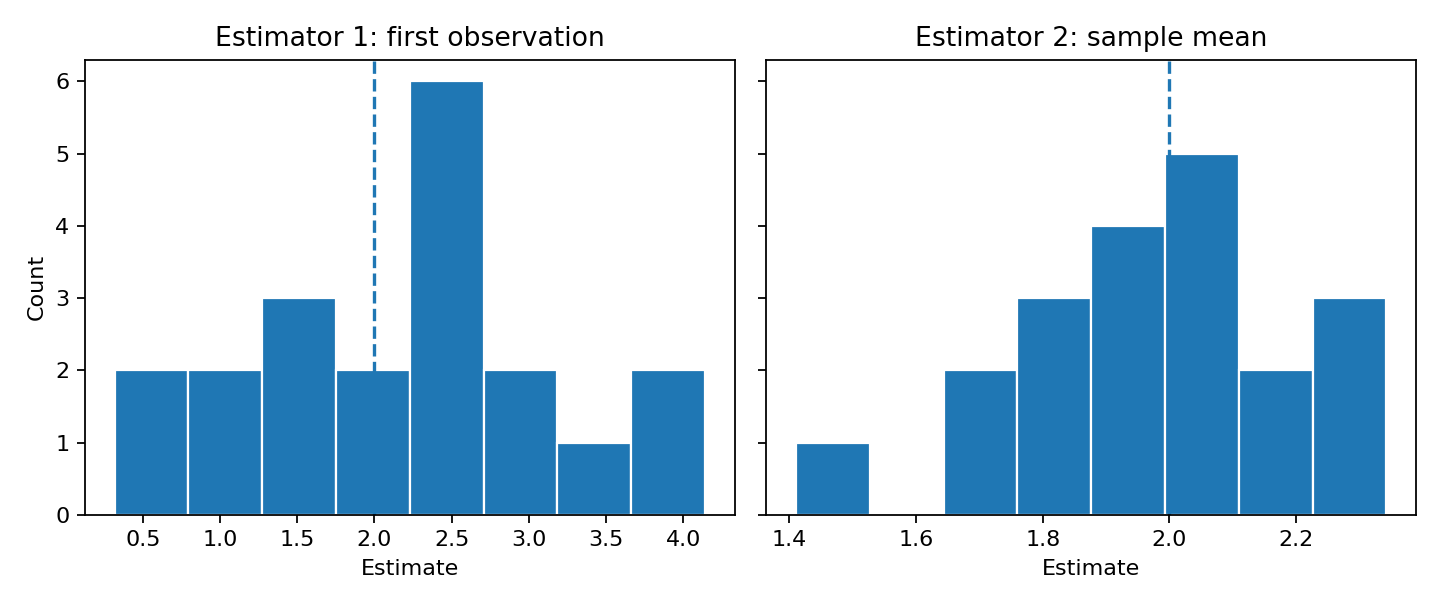
\includegraphics[width=0.88\textwidth]{code/output/exercise3_sampling_distributions.png}
\caption{Exercise 3 simulation. The sample mean has a much tighter sampling distribution than the first observation.}
\end{figure}

\subsubsection*{(d) Unbiasedness does not imply accuracy in every sample}
Unbiasedness is a statement about repeated sampling:
\[
 \E(\hat\mu)=\mu.
\]
It does not imply that $\hat\mu=\mu$ in a particular sample. A single draw can be far from the true mean because the estimator has sampling variance. Comparing only average estimates therefore hides the key difference between the two procedures: both are centered correctly, but $\bar Y$ has much smaller variance and is therefore much more precise.

\subsection{Exercise 4 -- Estimating the Error Variance}
Maintain SLR.1--SLR.5 and define
\[
 \Sxx=\sum_i(x_i-\bar x)^2,
 \qquad
 \SSR=\sum_i\hat u_i^2.
\]

\subsubsection*{(a) Decomposition of the residual sum of squares}
Start from
\[
 \hat u_i=u_i-(\hat\beta_0-\beta_0)-(\hat\beta_1-\beta_1)x_i.
\]
From Exercise 2,
\[
 d\equiv\hat\beta_1-\beta_1
 =\frac{\sum_i(x_i-\bar x)u_i}{\Sxx}.
\]
Also,
\[
 \hat\beta_0-\beta_0=\bar u-d\bar x.
\]
Therefore
\[
 \hat u_i=(u_i-\bar u)-d(x_i-\bar x).
\]
Squaring and summing,
\begin{align*}
 \SSR
 &=\sum_i(u_i-\bar u)^2
 -2d\sum_i(x_i-\bar x)(u_i-\bar u)
 +d^2\sum_i(x_i-\bar x)^2\\
 &=\sum_i u_i^2-n\bar u^2
 -2d\sum_i(x_i-\bar x)u_i+d^2\Sxx.
\end{align*}
Let $A=\sum_i(x_i-\bar x)u_i$, so $d=A/\Sxx$. Then
\[
 -2dA+d^2\Sxx=-\frac{A^2}{\Sxx}.
\]
Hence
\[
 \boxed{
 \SSR
 =\sum_i u_i^2-n\bar u^2
 -\frac{\left[\sum_i(x_i-\bar x)u_i\right]^2}{\Sxx}
 }.
\]

\subsubsection*{(b) Conditional expectation of SSR}
Under zero conditional mean and homoskedasticity,
\[
 \E(u_i\mid X)=0,
 \qquad
 \Var(u_i\mid X)=\sigma^2.
\]
Thus
\[
 \E\!\left(\sum_i u_i^2\mid X\right)=n\sigma^2.
\]
Since $\E(\bar u\mid X)=0$ and $\Var(\bar u\mid X)=\sigma^2/n$,
\[
 \E(n\bar u^2\mid X)=\sigma^2.
\]
Finally, for
\[
 A=\sum_i(x_i-\bar x)u_i,
\]
we have $\E(A\mid X)=0$ and
\[
 \Var(A\mid X)
 =\sigma^2\sum_i(x_i-\bar x)^2
 =\sigma^2\Sxx.
\]
Therefore
\[
 \E\!\left(\frac{A^2}{\Sxx}\middle|X\right)=\sigma^2.
\]
Putting the three terms together,
\[
 \boxed{\E(\SSR\mid X)=(n-2)\sigma^2}.
\]

\subsubsection*{(c) Bias of $\tilde\sigma^2=\SSR/n$}
\begin{align*}
 \E(\tilde\sigma^2\mid X)
 &=\frac{1}{n}\E(\SSR\mid X)\\
 &=\frac{n-2}{n}\sigma^2.
\end{align*}
Therefore
\[
 \boxed{\operatorname{Bias}(\tilde\sigma^2)
 =-\frac{2}{n}\sigma^2}.
\]
The estimator $\SSR/n$ is downward biased.

\subsubsection*{(d) Unbiased estimator and degrees of freedom}
Define
\[
 \hat\sigma^2=\frac{\SSR}{n-2}.
\]
Then
\[
 \E(\hat\sigma^2\mid X)
 =\frac{1}{n-2}(n-2)\sigma^2
 =\boxed{\sigma^2}.
\]
Two degrees of freedom are lost because the residuals are computed after estimating two regression parameters, $\beta_0$ and $\beta_1$. Equivalently, the residual vector satisfies two independent sample restrictions:
\[
 \sum_i\hat u_i=0,
 \qquad
 \sum_i x_i\hat u_i=0.
\]

\subsection{Exercise 5 -- Log-Level and Level-Log Specifications}
Assume variables inside logarithms are strictly positive.

\subsubsection*{(a) Change in a logarithm}
If $y_1=y_0+\Delta y$, then
\begin{align*}
 \Delta\log y
 &=\log(y_1)-\log(y_0)\\
 &=\log\!\left(\frac{y_0+\Delta y}{y_0}\right)\\
 &=\boxed{\log\!\left(1+\frac{\Delta y}{y_0}\right)}.
\end{align*}
For a small $r=\Delta y/y_0$, the first-order Taylor approximation $\log(1+r)\approx r$ gives
\[
 \boxed{\Delta\log y\approx\frac{\Delta y}{y_0}}.
\]

\subsubsection*{(b) Log-level model}
For
\[
 \log(y)=\beta_0+\beta_1x+u,
\]
a change $\Delta x$ changes the fitted log outcome by
\[
 \Delta\widehat{\log y}=\beta_1\Delta x.
\]
Thus the approximate percentage change is
\[
 \boxed{100\beta_1\Delta x\%}.
\]
Between exponentiated fitted log values,
\[
 \frac{\exp(\hat\ell_1)}{\exp(\hat\ell_0)}
 =\exp(\beta_1\Delta x),
\]
so the exact percentage change is
\[
 \boxed{100\left[\exp(\beta_1\Delta x)-1\right]\%}.
\]

\subsubsection*{(c) Level-log model}
For
\[
 y=\beta_0+\beta_1\log(x)+u,
\]
if $x$ increases by $p\%$, then
\[
 x_1=x_0\left(1+\frac{p}{100}\right).
\]
Therefore the exact change in fitted $y$ is
\[
 \boxed{
 \Delta\hat y
 =\beta_1\log\!\left(1+\frac{p}{100}\right)
 }.
\]
For a small percentage change,
\[
 \log\!\left(1+\frac{p}{100}\right)\approx\frac{p}{100},
\]
so
\[
 \boxed{\Delta\hat y\approx\beta_1\frac{p}{100}}.
\]

\subsubsection*{(d) Numerical applications}
For the log-level model with $\hat\beta_1=0.08$:
\begin{itemize}
 \item If $\Delta x=1$, the approximation is $8\%$, while the exact change is
 \[
 100(e^{0.08}-1)=\boxed{8.33\%}.
 \]
 \item If $\Delta x=4$, the approximation is $32\%$, while the exact change is
 \[
 100(e^{0.32}-1)=\boxed{37.71\%}.
 \]
\end{itemize}
For the level-log model with $\hat\beta_1=2.5$ and a $10\%$ increase in $x$,
\[
 \Delta\hat y_{\text{approx}}
 =2.5(0.10)=\boxed{0.25},
\]
whereas
\[
 \Delta\hat y_{\text{exact}}
 =2.5\log(1.10)
 =\boxed{0.2383}.
\]

\newpage
\section{Python Lab 1 -- Seeing Exogeneity and Bias by Simulation}
The supplied simulation keeps the same $x$ values and repeatedly estimates
\[
 y=1+0.5x+u
\]
under two data-generating processes:
\[
 \text{A: }u=\varepsilon,
 \qquad
 \text{B: }u=0.4x+\varepsilon,
 \qquad
 \varepsilon\sim N(0,4).
\]
The completed OLS slope function is the centered-sums formula
\[
 \hat\beta_1
 =\frac{\sum_i(x_i-\bar x)(y_i-\bar y)}
 {\sum_i(x_i-\bar x)^2}.
\]

\subsection*{(a) Sampling distributions and numerical output}
With $n=200$ and $5{,}000$ replications, the script produces:
\begin{center}
\begin{tabular}{lrr}
\toprule
Quantity & Case A & Case B\\
\midrule
Mean simulated slope & 0.502511 & 0.902511\\
Theoretical center & 0.500000 & 0.900000\\
\bottomrule
\end{tabular}
\end{center}
For Case A, the empirical variance of the slope is
\[
 0.0245403,
\]
while the theoretical conditional variance is
\[
 \frac{\sigma^2}{\Sxx}=0.0258426.
\]
The close agreement is what we expect from a large Monte Carlo experiment.

\begin{figure}[H]
\centering
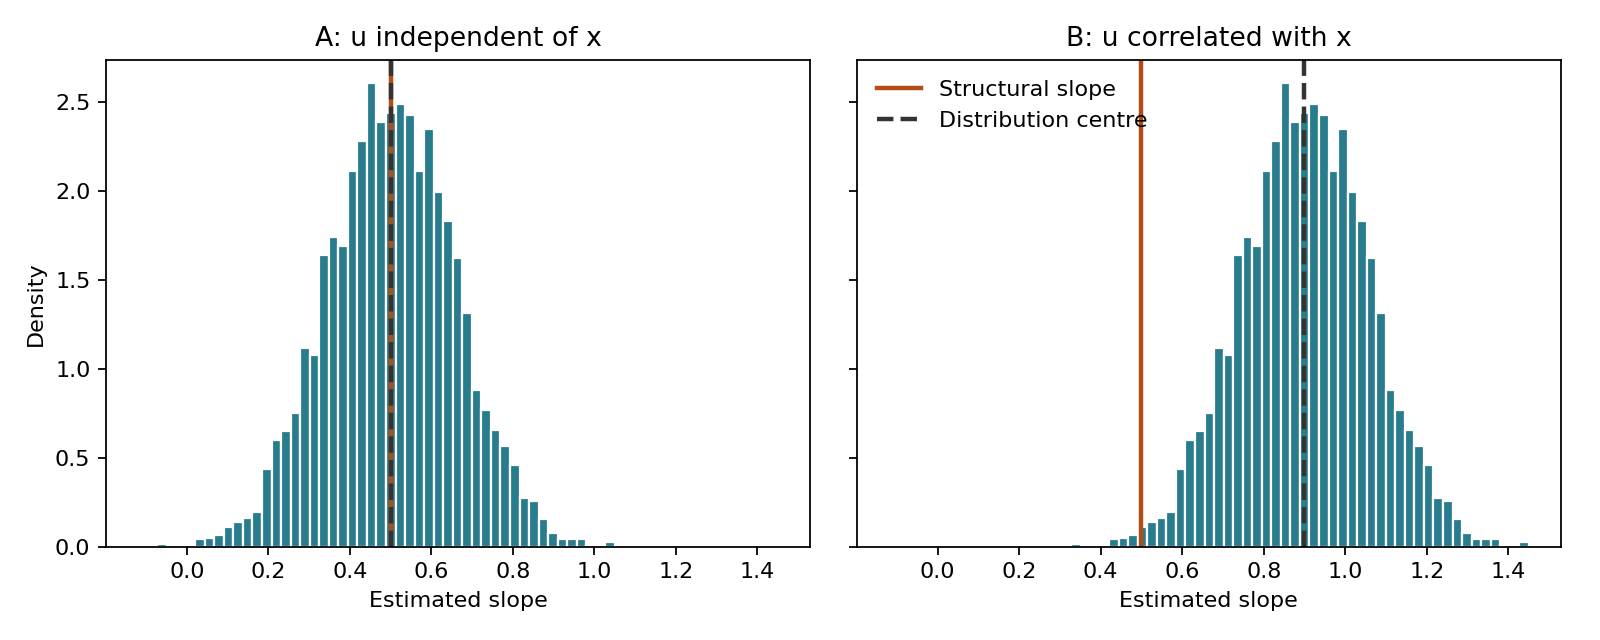
\includegraphics[width=0.92\textwidth]{code/output/lab1_sampling_distribution.png}
\caption{Sampling distributions of the OLS slope under exogeneity (A) and under correlation between $x$ and the error (B).}
\end{figure}

\subsection*{(b) Interpretation}
Under A, $\E(u\mid x)=0$, so the OLS slope is unbiased and its sampling distribution is centered at the structural slope $0.5$. A particular estimate can still be far from $0.5$ because unbiasedness concerns the average across repeated samples, not every realization.

Under B,
\[
 u=0.4x+\varepsilon
 \quad\Longrightarrow\quad
 \E(u\mid x)=0.4x\neq0,
\]
so zero conditional mean fails. Exercise 2 predicts
\[
 \E(\hat\beta_1\mid X)=0.5+0.4=0.9,
\]
which is exactly where the simulated distribution is centered. Increasing the number of Monte Carlo replications only estimates this biased sampling distribution more accurately; it does not move its center to $0.5$.

\newpage
\section{Python Lab 2 -- From Data to a Regression Interpretation}
The data contain 526 workers and 24 variables from the 1976 Current Population Survey. The analysis uses hourly wage (\texttt{wage}) and years of education (\texttt{educ}) and estimates simple regressions with education as the only explanatory variable.

\subsection{Step 1 -- Inspect Before Estimating}
\subsubsection*{(a) Data inspection}
The data have $526$ rows and $24$ columns. For the two variables used here:
\begin{center}
\begin{tabular}{lrr}
\toprule
Statistic & Wage & Education\\
\midrule
Count & 526 & 526\\
Mean & 5.8961 & 12.5627\\
Standard deviation & 3.6931 & 2.7690\\
Minimum & 0.5300 & 0\\
25th percentile & 3.3300 & 12\\
Median & 4.6500 & 12\\
75th percentile & 6.8800 & 14\\
Maximum & 24.9800 & 18\\
\bottomrule
\end{tabular}
\end{center}
There are no missing values in either variable. One observation represents one worker; wage is measured in 1976 US dollars per hour and education in years. The education range is $0$ to $18$ years.

\subsubsection*{(b) Mean, median, positivity, and regression sample}
The mean hourly wage is $5.8961$, whereas the median is $4.6500$. The mean exceeds the median because the wage distribution has a substantial right tail. The minimum wage is $0.53>0$, so all wages are strictly positive and the log wage can be computed. All $526$ observations are therefore used in every fitted model.

\subsubsection*{(c) Required two descriptive sentences}
\emph{One observation represents one worker; the sample contains 526 workers from the 1976 Current Population Survey. Wage is hourly earnings measured in 1976 US dollars, and education is measured in years.}

\subsection{Step 2 -- Visualise and Form a Prediction}
\subsubsection*{(a) Histograms and scatterplot}
\begin{figure}[H]
\centering
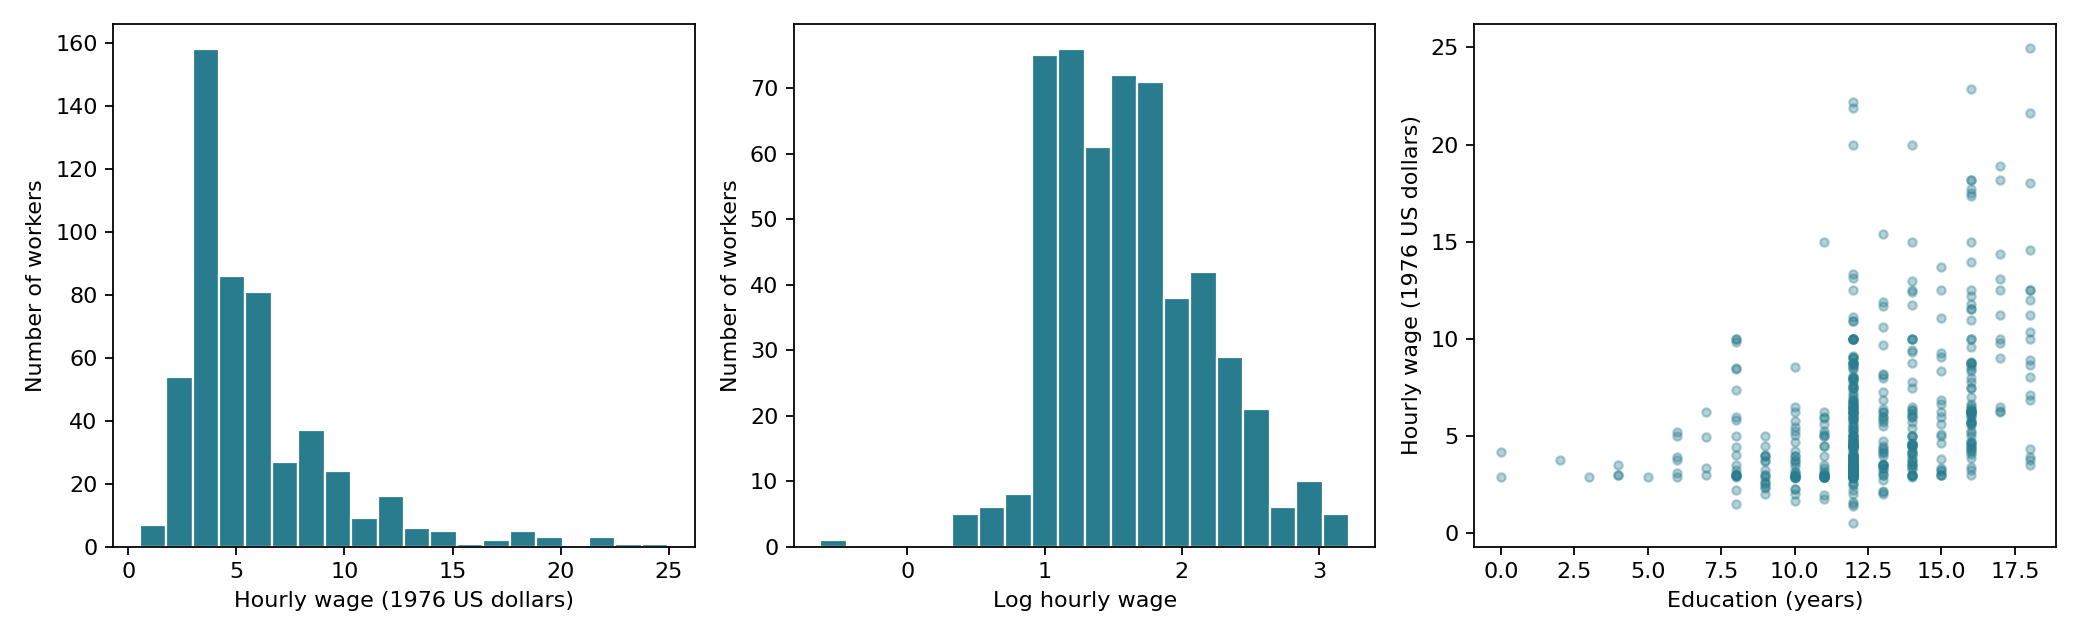
\includegraphics[width=\textwidth]{code/output/lab2_distributions_and_scatter.png}
\caption{Distribution of wage, distribution of log wage, and the wage--education scatterplot.}
\end{figure}
The wage histogram is strongly right-skewed, with a small number of high-wage observations. Logging wage compresses the upper tail and produces a much less skewed distribution. The scatterplot suggests a positive relationship between education and wage, but the vertical spread at a given education level is large.

\subsubsection*{(b) Correlation and predicted slope sign}
The sample correlation is
\[
 \boxed{\operatorname{Corr}(wage,educ)=0.4059}.
\]
Thus the simple-regression slope should be positive. The scatterplot does not suggest accurate prediction of every worker's wage because workers with the same or similar education levels can have very different wages.

\subsection{Step 3 -- Fit and Read a Simple Regression}
The estimated simple regression is
\[
 wage_i=a_0+a_1educ_i+v_i.
\]

\subsubsection*{(a) Coefficients, sample size, and $R^2$}
The software output gives
\[
 \hat a_0=-0.904852,
 \qquad
 \hat a_1=0.541359,
 \qquad
 n=526,
 \qquad
 R^2=0.164758.
\]
Rounded as requested,
\[
 \boxed{\widehat{wage}=-0.905+0.541\,educ},
 \qquad
 \boxed{n=526,\quad R^2=0.165}.
\]

\subsubsection*{(b) One and four additional years of education}
One additional year of education is associated with
\[
 \boxed{\$0.541\text{ more per hour}}.
\]
Four additional years are associated with
\[
 4(0.541359)=\boxed{\$2.165\text{ more per hour}}.
\]
This is a simple regression containing only education, so it does \emph{not} hold experience or any other worker characteristic fixed.

\subsubsection*{(c) Meaning of the negative intercept}
The negative intercept means that the fitted line predicts approximately $-\$0.905$ at zero years of education. It does not imply that all fitted wages are negative, because fitted wage increases by about $0.541$ for each additional year of education. The intercept is mainly the location where the fitted line crosses the vertical axis and is not economically useful here as a literal wage prediction.

\subsubsection*{(d) Centered-sums calculation and fitted line}
Using the centered-sums formula gives
\[
 \hat a_1
 =\frac{\sum_i(educ_i-\overline{educ})(wage_i-\overline{wage})}
 {\sum_i(educ_i-\overline{educ})^2}
 =0.5413592547,
\]
and
\[
 \hat a_0=\overline{wage}-\hat a_1\overline{educ}
 =-0.9048516120.
\]
These match the software coefficients up to numerical precision.

\begin{figure}[H]
\centering
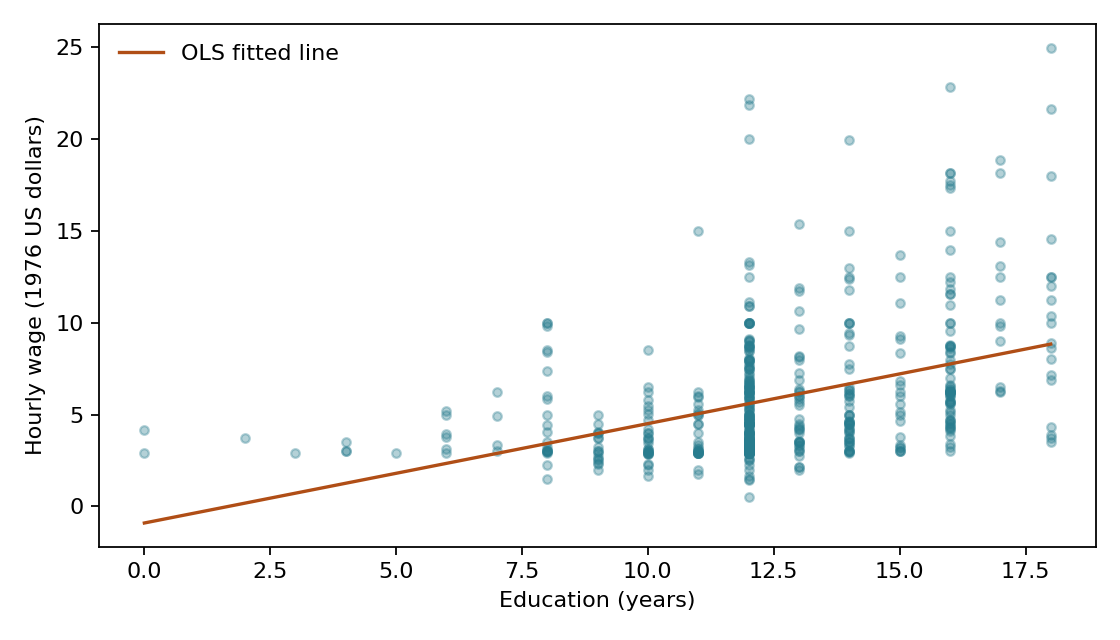
\includegraphics[width=0.82\textwidth]{code/output/lab2_fitted_line.png}
\caption{Observed hourly wages and the OLS fitted line.}
\end{figure}

\subsubsection*{(e) Required two interpretation sentences}
\emph{One additional year of education is associated with an estimated $\$0.541$ increase in hourly wage. Education is the only included regressor, so no other worker characteristic is held fixed and the estimated relationship is an association, not a causal effect.}

\subsection{Step 4 -- Fitted Values and Residuals}
\subsubsection*{(a) Fitted wages at 12 and 16 years of education}
The fitted values are
\[
 \widehat{wage}(12)=\boxed{5.591459},
 \qquad
 \widehat{wage}(16)=\boxed{7.756896}.
\]
Their difference is
\[
 7.756896-5.591459=\boxed{2.165437},
\]
which is exactly four times the estimated slope. These are fitted values from the regression line, not the known wage of every worker with 12 or 16 years of education.

\subsubsection*{(b) First residual}
For the first observation, $educ_1=11$ and $wage_1=3.10$. The fitted wage is
\[
 \widehat{wage}_1=5.050100,
\]
so
\[
 \hat u_1=wage_1-\widehat{wage}_1
 =3.10-5.050100
 =\boxed{-1.950100}.
\]
The residual is negative because this worker's actual wage lies below the fitted regression line. We can calculate the residual because the fitted coefficients are observed after estimation; we cannot calculate the population error $u_i$ because the true population regression function and its true coefficients are unknown.

\subsubsection*{(c) OLS checks}
Numerically,
\[
 \sum_i\hat u_i=-4.01\times10^{-12}\approx0.
\]
Also,
\[
 \widehat{wage}(\overline{educ})=5.896102675,
 \qquad
 \overline{wage}=5.896102675.
\]
Thus the residuals sum to zero up to floating-point error and the fitted line passes through $(\overline{educ},\overline{wage})$. These facts do not validate exogeneity; they are mechanical consequences of OLS with an intercept.

\subsubsection*{(d) Residual plot}
\begin{figure}[H]
\centering
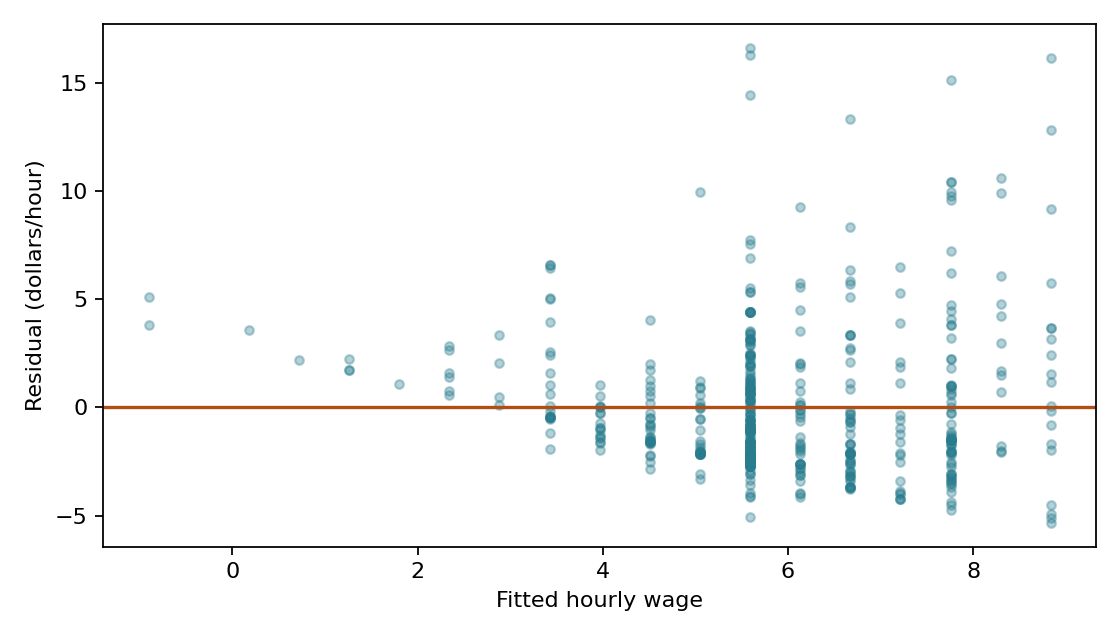
\includegraphics[width=0.82\textwidth]{code/output/lab2_residuals.png}
\caption{OLS residuals plotted against fitted hourly wages.}
\end{figure}
The residual spread appears to become wider at larger fitted wages, especially on the positive side. This is a descriptive visual pattern that may suggest non-constant variance, but the plot is not a formal test and it does not prove a causal problem.

\subsubsection*{(e) Required fitted-value sentence}
\emph{At 12 years of education the regression predicts an hourly wage of about $\$5.59$, which is a fitted value from the sample regression and not the actual wage of every worker with 12 years of education.}

\subsection{Step 5 -- Compare Specifications and Units}
The three fitted models are
\[
 \text{A: } wage_i=a_0+a_1educ_i+v_i,
\]
\[
 \text{B: } \log(wage_i)=b_0+b_1educ_i+e_i,
\]
\[
 \text{C: } wage\_cents_i=c_0+c_1educ_i+w_i,
 \qquad wage\_cents_i=100wage_i.
\]

\subsubsection*{(a) Model comparison table}
\begin{center}
\begin{tabular}{p{1.4cm}p{1.8cm}rrrp{3.2cm}r}
\toprule
Model & Outcome & Intercept & Slope & $R^2$ & Slope units & $n$\\
\midrule
A & wage & -0.904852 & 0.541359 & 0.164758 & dollars/hour/year & 526\\
B & log wage & 0.583773 & 0.082744 & 0.185806 & log points/year & 526\\
C & wage cents & -90.485161 & 54.135925 & 0.164758 & cents/hour/year & 526\\
\bottomrule
\end{tabular}
\end{center}
All three models use $n=526$. The slopes from A and B cannot be compared as dollar amounts because they refer to different outcome units: Model A uses wage levels in dollars per hour, whereas Model B uses log wage.

\subsubsection*{(b) Approximate and exact percentage comparison in Model B}
For one additional year of education,
\[
 100\hat b_1
 =100(0.0827444)
 =\boxed{8.274\%}.
\]
The exact percentage difference between exponentiated fitted log wages is
\[
 100\left(e^{\hat b_1}-1\right)
 =\boxed{8.626\%}.
\]
Applying the same exact percentage to the conditional arithmetic mean $\E(wage\mid educ)$ requires the retransformation factor
\[
 \E(e^e\mid educ)
\]
to be constant in education (for example, this follows if the distribution of the log error is independent of education). Without such a restriction, exponentiating a fitted log value does not by itself give the conditional arithmetic mean wage.

\subsubsection*{(c) Exponentiated fitted log wages}
At 12 years of education,
\[
 \widehat{\log(wage)}=1.576705,
 \qquad
 e^{1.576705}=\boxed{4.838985}.
\]
At 16 years,
\[
 \widehat{\log(wage)}=1.907683,
 \qquad
 e^{1.907683}=\boxed{6.737457}.
\]
These are \emph{exponentiated fitted log wages}. They should not automatically be called estimates of mean wages because generally
\[
 \E(wage\mid educ)
 =e^{\beta_0+\beta_1educ}\E(e^e\mid educ),
\]
and the final expectation need not equal one.

\subsubsection*{(d) Comparing the two $R^2$ values}
Model B has $R^2=0.185806$, larger than Model A's $0.164758$, but this does not establish that B predicts wage in dollars better. The two $R^2$ statistics use different dependent variables and therefore different total sums of squares:
\[
 \sum_i(wage_i-\overline{wage})^2
 \quad\text{versus}\quad
 \sum_i(\log wage_i-\overline{\log wage})^2.
\]
They measure fractions of variation on different scales and are not directly comparable for dollar prediction performance.

\subsubsection*{(e) Changing dollars to cents}
Since $wage\_cents=100\,wage$, we expect the intercept, slope, fitted values, and residuals to be multiplied by 100, while $R^2$ remains unchanged. The estimates confirm this:
\[
 -90.485161=100(-0.904852),
 \qquad
 54.135925=100(0.541359),
\]
and the numerical checks for coefficients, residuals, and $R^2$ are all \texttt{True}. Expressing wages in cents changes only the units and provides no new economic information.

\subsubsection*{(f) Required three sentences}
\emph{In Model A, one additional year of education is associated with about $\$0.541$ more hourly wage. In Model B, one additional year is associated with approximately $8.274\%$ higher wage and with an exact $8.626\%$ difference between exponentiated fitted log wages. Neither estimate is automatically causal because education is the only included regressor and omitted factors such as ability can be related to both education and wages.}

\section{Key Output Files Generated by the Completed Script}
The completed script generates the following files in \texttt{code/output/}:
\begin{itemize}
 \item \texttt{exercise3\_sampling\_distributions.png}
 \item \texttt{exercise3\_comparison.csv}
 \item \texttt{lab1\_sampling\_distribution.png}
 \item \texttt{lab2\_distributions\_and\_scatter.png}
 \item \texttt{lab2\_fitted\_line.png}
 \item \texttt{lab2\_residuals.png}
 \item \texttt{lab2\_predictions.csv}
 \item \texttt{lab2\_specifications.csv}
 \item \texttt{console\_output.txt}
\end{itemize}

\appendix
\section{Complete Python Console Output}
\lstinputlisting{code/output/console_output.txt}

\section{Completed Python Script}
\lstinputlisting[language=Python]{code/lab1.py}

\end{document}
